

%%%%%%%% 
%%%%%%%% DO NOT CHANGE ANYTHING FROM HERE 
%%%%%%%% 
\documentclass[a4paper,UKenglish,cleveref, autoref, thm-restate]{lipics-v2021}
%This is a template for producing LIPIcs articles. 
%See lipics-v2021-authors-guidelines.pdf for further information.
%for A4 paper format use option "a4paper", for US-letter use option "letterpaper"
%for british hyphenation rules use option "UKenglish", for american hyphenation rules use option "USenglish"
%for section-numbered lemmas etc., use "numberwithinsect"
%for enabling cleveref support, use "cleveref"
%for enabling autoref support, use "autoref"
%for anonymousing the authors (e.g. for double-blind review), add "anonymous"
%for enabling thm-restate support, use "thm-restate"
%for enabling a two-column layout for the author/affilation part (only applicable for > 6 authors), use "authorcolumns"
%for producing a PDF according the PDF/A standard, add "pdfa"

%\graphicspath{{./graphics/}}%helpful if your graphic files are in another directory
\usepackage[utf8]{inputenc}
\usepackage{graphicx} %package to manage images
\graphicspath{ {./images/} }


\usepackage[rightcaption]{sidecap}

\usepackage{wrapfig}
\bibliographystyle{plainurl}% the mandatory bibstyle

%%%%%%%% 
%%%%%%%% DO NOT CHANGE UNTIL HERE
%%%%%%%% 

%%%%%%%% 
%%%%%%%% INCLUDE YOUR LATEX PACKAGES: READ AUTHOR GUIDELINES BEFORE
%%%%%%%% 

%%%%%%%% 
%%%%%%%% ADD YOUR OWN LATEX COMMANDS, IF NEEDED
%%%%%%%% 

%%%%%%%% 
%%%%%%%% ADD YOUR PERSONAL DATA AND TITEL
%%%%%%%% 

\title{A Survey on Machine Learning Benchmarks and their Application Domains } %TODO Please add

\titlerunning{} %TODO optional, please use if title is longer than one line

\author{Priya Shukla}{Ulm University, Germany}{Priya.shukla@uni-ulm.de}{}{}%TODO mandatory, please use full name; only 1 author per \author macro; first two parameters are mandatory, other parameters can be empty. Please provide at least the name of the affiliation and the country. The full address is optional

\authorrunning{P Shukla} %TODO mandatory. First: Use abbreviated first/middle names. Second (only in severe cases): Use first author plus 'et al.'

\Copyright{Ulm University} %TODO mandatory, please use full first names. LIPIcs license is "CC-BY";  http://creativecommons.org/licenses/by/3.0/

%%%%%%%% 
%%%%%%%% FOR THE CAMERA READY VERSION, SELECT THE CCDESC AND 3-5 KEYWORDS
%%%%%%%% 

\ccsdesc[100]{\textcolor{black}{Computing methodologies → Machine learning; Security and privacy; Hardware → Emerging technologies; Applied computing → Physical sciences and engineering}}
%TODO mandatory: Please choose ACM 2012 classifications from https://dl.acm.org/ccs/ccs_flat.cfm 

\keywords{Machine learning, Benchmarks, Deep learning, DNN, Neural Networks, Random Forest, K-nearest neighbour} %TODO mandatory; please add comma-separated list of keywords

%%%%%%%% 
%%%%%%%% DO NOT CHANGE ANYTHING FROM HERE 
%%%%%%%% 

%\category{} %optional, e.g. invited paper

%\relatedversion{} %optional, e.g. full version hosted on arXiv, HAL, or other respository/website
%\relatedversiondetails[linktext={opt. text shown instead of the URL}, cite=DBLP:books/mk/GrayR93]{Classification (e.g. Full Version, Extended Version, Previous Version}{URL to related version} %linktext and cite are optional

%\supplement{}%optional, e.g. related research data, source code, ... hosted on a repository like zenodo, figshare, GitHub, ...
%\supplementdetails[linktext={opt. text shown instead of the URL}, cite=DBLP:books/mk/GrayR93, subcategory={Description, Subcategory}, swhid={Software Heritage Identifier}]{General Classification (e.g. Software, Dataset, Model, ...)}{URL to related version} %linktext, cite, and subcategory are optional

\funding{}%optional, to capture a funding statement, which applies to all authors. Please enter author specific funding statements as fifth argument of the \author macro.

%\acknowledgements{I want to thank \dots}%optional

\nolinenumbers %uncomment to disable line numbering

\hideLIPIcs  %uncomment to remove references to LIPIcs series (logo, DOI, ...), e.g. when preparing a pre-final version to be uploaded to arXiv or another public repository

%Editor-only macros:: begin (do not touch as author)%%%%%%%%%%%%%%%%%%%%%%%%%%%%%%%%%%
\EventEditors{}
\EventNoEds{1}
\EventLongTitle{)}
\EventShortTitle{}
\EventAcronym{}
\EventYear{}
\EventDate{}
\EventLocation{}
\EventLogo{}
\SeriesVolume{}
\ArticleNo{}
%%%%%%%%%%%%%%%%%%%%%%%%%%%%%%%%%%%%%%%%%%%%%%%%%%%%%%

%%%%%%%% 
%%%%%%%% DO NOT CHANGE UNTIL HERE
%%%%%%%% 

\begin{document}

\maketitle

%TODO mandatory: add short abstract of the document
\begin{abstract}
There is a lot of considerable research on systems, algorithms and hardware to speed up and find accurate results for a machine learning problem. With a lot of data available on the internet, it is easier to access information, database, and tools to perform research. Since there are multiple methods to train the software, we need to find the best out of them. The paper surveys seventeen research papers and findings related to machine learning benchmarks. Historically for modelling and simulation of high-performance computing systems, the issues have been addressed through benchmarking computer applications, algorithms and architectures. The paper explains how benchmarking works in machine learning by focusing on scientific benchmarking, application or system benchmarking. Also, the paper lists different benchmarking libraries, suites and methods to develop the best solution. The survey compares the benchmark suites and finds the best based on categories, metrics, framework, reporting and compliance, data, coverage, distribution, and extensibility. Further, the benchmarking of accelerators provides insights in terms of power consumption and speed. There are fields where we can tell the best machine learning method by benchmarking them on their datasets. Hence the paper discusses those applications like photometric redshifts of galaxies, frauds in credit card transactions, short-term PV(photoVoltaic)-power forecasting, protein classification, and seizure type classification.
\end{abstract}

\section{ Introduction}
\label{introduction}
 
We come across multiple artificial intelligence in our daily life like Alexa, Siri, self-driving cars, recommendations on Netflix, Facial Filters Instagram) etc. AI and machine learning (ML) have revolutionized many industries, militaries, and other organizations. Machine learning is a subset of Al where we train the machine(computers) where it learns from the experiences. It addresses the challenges of evolving events, data deluge, and rapid courses of action~\cite{accele}. We have many frameworks, but not every framework fits best in all situations so we need to benchmark them and evaluate their performance.

Benchmarking the methods and evaluating them on certain parameters such as the size of the training set, modern hardware platforms, transfer learning, extrapolation on the prediction accuracy, and training and inference times yield the best output~\cite{sctmlb}. Now, if we have huge data we can perform machine learning and automate the future response. The above statement is true in banking, medicine, physics, research, astronomy, and day-to-day electronic devices, etc. Every field has a large number of datasets thus we can automate and develop faster and better solutions with machine learning. While each problem statement and the datasets are unique hence the process and solution will also be unique. The survey includes ongoing research and published results related to the benchmarking of machine learning methods. 

The following work will provide an overview of the topic and is structured as follows: 

Section \ref{related work} mentions the related work. Section \ref{benchmarks} covers the categories of benchmarks based on the goals, requirements to develop a solution, and challenges addressed to find the best solution. Section \ref{machine learning frameworks} briefs the framework whereas section \ref{benchmarking suites} lists benchmark suites and compares them based on challenges, categories, and requirements mentioned in section \ref{machine learning frameworks}. Section \ref{Benchmarking the accelerators} has findings for benchmarking the accelerators. Section \ref{applications of Benchmarks} has listed the real-time examples. Finally, section \ref{Discussion} and section \ref{conclusion} discuss the major findings and concluded the survey.

\section{Related work}
\label{related work}
In this section, we will review some of the existing surveys on benchmarking machine learning and its applications:
\begin{enumerate}
\item Albert et al.~\cite{accele} focused on benchmarking the hardware by considering power consumption and performance of processors and hardware as important parameters. It is further discussed in section \ref{Benchmarking the accelerators}.
\item In the research paper~\cite{casesynthesizing} the main focus is to reevaluate CLgen\footnote{An open source application for generating runnable programs using deep learning \url{https://pythonlang.dev/repo/chriscummins-clgen/}}. Their dataset shows dataset derived from the mined GitHub kernels yields better results than the synthetic one produced by the generative model of code based on LSTM\footnote{Long Short-Term Memory}, proposed by Cummins et al~\cite{cuminsetal}.
\item  Shankar et al.~\cite{sctmlb} focused on the scientific machine learning benchmarks, however, we have other categories also like application and system benchmarking which can be seen in section \ref{benchmarks}.
\item Mark et al.~\cite{randomforestregression} discussed the formulation of random forests and investigates prediction and performance on real-world and simulated datasets for which maximally sized trees do overfit. We discuss its major finding in our discussion section \ref{Discussion}.
Apart from the above surveys and benchmarking research, we have some complex problems being solved by machine learning. We can find the random forest algorithm performing best in the application section \ref{applications of Benchmarks}.
\item Giang et al.~\cite{RefWorksframework} have discussed the detailed evolution, and analysis of machine learning and deep learning frameworks. The paper has a detailed comparison of various metrics including hardware parameters.
\item Lucas et al.r~\cite{decodingmlb} talk about decoding the machine learning benchmarks. It states that IRT(Item Response Theory)\footnote{\url{https://edres.org/irt/}} can tell which is a good benchmark.

Above are some existing works and being a survey we include the above findings in our paper.
\end{enumerate}
\section{Benchmarks}
\label{benchmarks}
 Supervised, unsupervised and reinforcement learning are three approaches for developing machine learning-based solutions.
\begin{figure}[ht]
    \centering
    \includegraphics[width=13cm]{images/benchmark.PNG}
    \caption{ The notion of a machine learning benchmark and a benchmark suite. a | Elements of
a scientific machine learning (ML) benchmark. b | Building a scientific ML benchmark suite that
integrates different scientific ML benchmarks from various scientific disciplines~\cite{sctmlb}.}
    \label{fig:figure 1}
\end{figure}
When we train a computer algorithm on input data that has labelled output then it is called Supervised Learning. Pattern classification or estimation is the real-time usage of supervised learning~\cite{sctmlb}.  In unsupervised learning, the algorithms identify patterns in unclassified and unlabelled data sets. Reinforcement Learning works on a trial-and-error approach and it rewards the system with correct output and penalizes it for wrong output~\cite{RefWorksreinforcement}.  
It is a complex and time-consuming process to find a perfect algorithm. We consider the following factors to make the process easier~\cite{sctmlb}:
 \begin{enumerate}
\item Type, quantity and quality of the training data.
\item Availability of labelled data.
\item The type of problem being addressed (prediction, classification and so on).
\item Overall accuracy and performance required.
\item Hardware systems available for training and inferencing. 
 \end{enumerate}
Creating a benchmark for any problem requires two major elements. Dataset: On which this benchmark is trained or inferences upon, and other is a reference implementation, for example- any programming language such as Python, C++, etc.  A collection of such benchmarks can make up a benchmark suite, as illustrated in
Figure \ref{fig:figure 1}.

\subsection{Categories of Benchmarking}
\label{categories of benchmarking}
By considering ML benchmarks as models for use in a variety of scientific problems, different aspects of an ML ecosystem can be compared and contrasted. Now we will discuss different types of benchmarks based on our focus and target which can be categorised as Scientific ML Benchmarking, Application Benchmarking, and System Benchmarking as discussed below.

 
     \subsubsection{Scientific ML Benchmarking}
     \label{scientific ml benchmarking}
    In this type, the testing of algorithms and their performance is done on fixed datasets in the same hardware and software environment. The characteristics of this benchmark are the datasets with some specific scientific objective. To perform different methods of analysis and exploration requires rich data obtained from a scientific experiment.
     
F1 score for training accuracy and time to solution, inferring the structure of multiphase materials from X-ray diffuse multiple scattering data,  estimating the photometric redshifts of galaxies(discussed in the application section \ref{applications of Benchmarks}), clustering of microcracks in a material using X-ray scattering data, and removing noise from microscope data to improve the quality of images are some of the examples of this benchmarking~\cite{sctmlb}.
    \subsubsection{Application Benchmarking}
    \label{application benchmarking}
     
This aspect of ML benchmarks is concerned with the end-to-end performance of the complete ML application (covering loading of inputs from files, pre-processing, application of ML, post-processing and writing outputs to files) on different hardware and software environments.
We can also evaluate the performance of particular hardware, library, run environments, file systems or overall systems.
Throughput measures like images per second could be one of the metrics in the case of image classification for training or inference. The time to solution of the classification problem (including I/O, ML, and pre-processing and post-processing) or the scaling properties of the application are examples of metrics in this benchmarking ~\cite{sctmlb}.

    \subsubsection{System Benchmarking}
    \label{system benchmarking}
     In this type, the concern is to investigate the performance effects of the system hardware architecture on improving the scientific outcomes or targets. It could be confused with application benchmarking, so to differentiate one has to focus on a specific operation that exercises a particular part of the system, independent of the broader system environment.
The example metrics are the time to solution, the number of floating-point operations per second achieved or aspects of network and data movement performance.


\subsection{Requirements}
\label{requirements}
Since the process of benchmarking is quite complex, we require some of the following elements to find the best solution:
\begin{enumerate}

\item \textbf{Metrics of choice -}
As mentioned some metrics in the categories of benchmarking, for all the problems we need some metrics to compare the performance.
In scientific benchmarking, the metric will vary as per the benchmarks. However, in system-level benchmarking, we may find common metrics over a range of applications. 
However, in the context of ML, because of the uncertainty across the underlying ML models, datasets and device hardware, we need to compare and quantify the uncertain outputs~\cite{sctmlb}.

\item \textbf{Framework -}
A set of complex benchmarking operations is performed to achieve the goal. Hence we search the framework and achieve the goals of benchmarking suites to unify the benchmark portability, flexibility, and logging~\cite{sctmlb}.

\item \textbf{Reporting and compliance -}
It is important to report the results and most of the suites address it. However, in case of specific compliances, we need to include it in the suites for example ensuring that the process is carried out fairly across different hardware platforms~\cite{sctmlb}.

\item \textbf{Latency -} 
Latency refers to the time taken to process one unit of data provided only one unit of data is processed at a time. The goal is to minimize latency as opposed to throughput on CPUs~\cite{sctmlb}.
\end{enumerate}

\subsection{Challenges}
\label{Challenges}
We should also address the below-mentioned challenges when dealing with the development of ML benchmarks:
\begin{enumerate}

\item \textbf{Data -} 
We need a wide range of curated, large-scale, scientific datasets. It could be experimental or simulated data coupled with the relevant applications. We can lose access and control of external datasets. Hence maintenance and distribution of large-scale datasets for public consumption is a challenging process~\cite{sctmlb}.

\item \textbf{Distribution - }
The users must have access to relevant datasets and reference implementation. However, downloading such large-size datasets
is a major challenge~\cite{sctmlb}.

\item \textbf{Coverage -}  
Covering all the elements mentioned above is a big challenge for any benchmark. Thus ideally benchmarks should focus on providing good coverage of methods and goals and should be extensible~\cite{sctmlb}.

 \item \textbf{Extensibility -} 
 Developing benchmarks is a time-consuming process. A good benchmarking framework should minimize the amount of code refactoring required for conversion into a benchmark as it is not efficient if the original application needs substantial refactoring~\cite{sctmlb}.
 
\end{enumerate}

Also overtraining and overfitting are the challenges which can be covered by requiring compliance with some general rules for the benchmarks such as specifying the set of hyperparameters that are open to tuning.
For example, the training and validation data, and cross-validation procedures, should aim to mitigate the dangers of overfitting~\cite{sctmlb}.

\section{Machine Learning Frameworks}
\begin{figure}[ht]
    \centering
    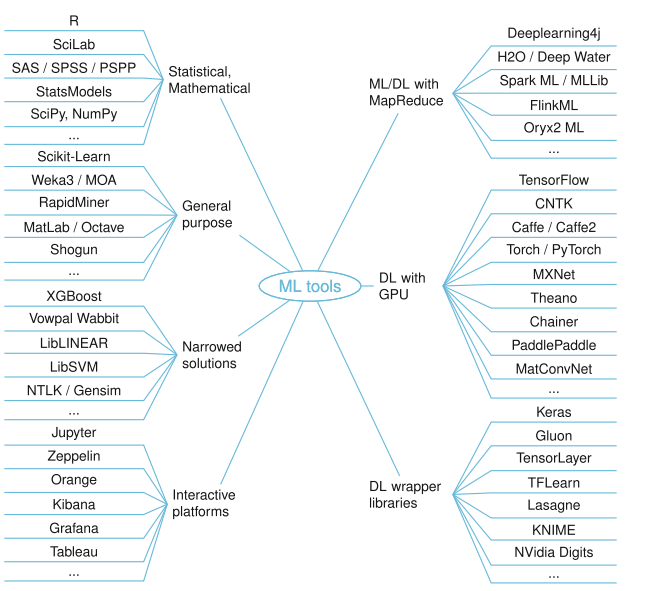
\includegraphics[width=13cm]{images/frameworks.PNG}
    \caption{ Overview of Machine Learning frameworks and libraries
Choosing framework is a difficult task and depends on the requirements and metrics discussed above~\cite{RefWorksframework}.}
    \label{fig:framework}
\end{figure}
\label{machine learning frameworks}
The number of ML algorithms, as well as
 their different software implementations, are quite
large.
Many software tools for DM using ML techniques have been in development for the past
25 years~\cite{RefWorksframework}, however, it is important to understand that all the frameworks have different areas of focus, one framework can not solve all the problems.
In the application section \ref{applications of Benchmarks} we have compared the Random Forest\footnote{\url{https://www.ibm.com/cloud/learn/random-forest}}, k-Nearest Neighbours\footnote{\url{https://www.ibm.com/topics/knn}}, Support Vector Machine(SVM)\footnote{\url{https://scikit-learn.org/stable/modules/svm.html}}, Artificial Neural Network\footnote{\url{https://www.sciencedirect.com/topics/earth-and-planetary-sciences/artificial-neural-network}}, Boosted Decision Trees\footnote{\url{https://xgboost.readthedocs.io/en/stable/tutorials/model.html}}, 1NN, Stochastic Gradient Descent (SGD)\footnote{\url{https://scikit-learn.org/stable/modules/sgd.html}}, XGBoost, and Convolutional Neural Networks (CNN)\footnote{\url{https://journalofbigdata.springeropen.com/articles/10.1186/s40537-021-00444-8}} based on the focus and problem statement and stated the best-performing ones.
 
    The above-mentioned are some of the tools which can be used based on the above-mentioned categories, requirements and to overcome the challenges.
  There are many frameworks available for Machine learning and Deep learning for example in the above Figure \ref{fig:framework}.

\section{Benchmarking Suites}
\label{benchmarking suites}
ML
benchmarks are commonly used to explore how far ML algorithms can go while
handling datasets~\cite{decodingmlb}.
Now we can have a look at different benchmark suites and compare them on the basis of discussed categories, requirements and challenges in Figure \ref{fig:benchmarkassessment}:
\subsection{Deep500}
\label{Deep500}
    A customizable infrastructure that enables detailed, accurate, fast, and fair benchmarking of DL codes. It can independently extend and benchmark DL procedures related to simple operators, whole neural networks, training schemes, and distributed training. It can accommodate a wide variety of techniques and methods. The principles behind this design can be reused to enable interpretable and reproducible benchmarking of extreme-scale codes in domains outside DL~\cite{deep500}.  However, the new benchmark development can't be adopted out of this one as it works on mapping a code to a new framework. The lack of a suite
of representative benchmarks is its main limitation and it doesn't include neural networks and a customizable framework, benchmarks or applications. The support of reporting is also left to the end-user hence failing to overcome section \ref{requirements}~\cite{sctmlb}.

    \subsection { CORAL-2}
    \label{Coral2}
    The CORAL-2~\cite{RefWorkscoral2} benchmark is backed by community code and by a scientific domain or data science. It includes majorly two suites big data analytics (BDAS) and Deep Learning (DLS) hence limited to DLS, BDAS and data distribution for algorithm improvement. The users have to evaluate and optimize the code to demonstrate their findings on a benchmark suite relevant to computational scientists. Principal components analysis (PCA), k-means clustering and SVM are included in the BDAS suite whereas the DLS suite relies on ImageNet\footnote{\url{https://image-net.org/}} and CANDLE\footnote{\url{https://proxyapps.exascaleproject.org/app/candlebm/}} benchmarks are primarily used for testing scalability aspects. It fails to address data, distribution, and extensibility.~\cite{sctmlb}.


    \subsection{ RLBench}
    \label{rlbench}
    It features unique and hand-crafted tasks as a benchmark and learning environment. 	New algorithmic
developments are evaluated with the set of tasks around reinforcement learning,
imitation learning, multitask learning,
geometric computer vision and,
few-shot learning.
It lacks the support for scientific benchmarking and comparison of the frameworks with coherent goals~\cite{sctmlb}.


\subsection{AIBench}
\label{AIbench}
It is
supported by the International Open
Benchmark Council (BenchCouncil)\footnote{\url{https://www.benchcouncil.org/conferences.html}}~\cite{RefWorkaiBenchmark}.
It focuses broadly on internet services such as search engines, social networks and e-commerce. Image classification, image generation, translation (image-to-text, image-to-image, text-to-image, text-to-text), object detection, text summarization, advertising and natural language processing are some ML-specific tasks performed by this suite. This suite partially addresses the challenges. It addresses several scientific problems from various domains. Extreme weather analysis is one of its real-world scientific DL applications. It reports the ranking information of hardware systems hence abiding by major levels of compliance.
~\cite{sctmlb}.
\subsection{DAWNBench}
\label{Dawnbench}
It is a suite for end-to-end DL training and inference hence making it ideal for application-level and system-level benchmarking. A benchmark and competition focused on end-to-end training time to achieve a state-of-the-art accuracy level, as well as inference time with that accuracy. Image classification (using the ImageNet and CIFAR-10\footnote{\url{https://www.cs.toronto.edu/~kriz/cifar.html}} ~\cite{RefWorksdawnBench:} datasets) and natural language-processing-based question answering~\cite{RefWorksdawnBench:} (based on the Stanford Question Answering Dataset or SQuAD\footnote{\url{https://rajpurkar.github.io/SQuAD-explorer/}}~\cite{RefWorksdawnBench:}) are its major benchmarks suites. DAWNBench evaluates deep learning systems on different tasks based on several metrics, using multiple datasets. Reasoning about deep learning systems in this way exposes valuable trade-offs between training time, training cost, and inference time.
It does not offer the notion of a framework, does not have a focus on science, and fails to provide distribution mechanisms~\cite{RefWorksdawnBench:}.
\subsection{SciMLBench(Scientific Machine Learning Benchmark)}
\label{SciMLBench}
It is designed for easy extensibility and its key focus is scientific ML. It is written in Python and is a full-fledged application. It offers a set of APIs with layers of abstraction and is organized into specific themes, including DL-focused benchmarks. It is compliant with the compliant with respect the FAIR guidelines (Findable, Accessible, Interoperable and Reusable). The framework serves at the user and developer levels~\cite{RefWorksdawnBench:}.

\begin{figure}[ht]
    \centering
    \includegraphics[width=14 cm]{images/benchmark assessment.PNG}
    \caption{ Overall assessment of various scientific machine learning benchmarking approaches
 In qualitatively assessing how far each approach addresses the concerns, we have indicated whether they offer no support (none), partial or questionable support
(partial) or fully support the concern (full)~\cite{sctmlb}.}
    \label{fig:benchmarkassessment}
\end{figure}

However, the above benchmarks can be used based upon the required parameters, there is no standard evaluation strategy yet capable of pointing out which is the best set of datasets to serve
as the gold standard to test different ML algorithms. In recent studies, Item
Response Theory (IRT) has emerged as a new approach to elucidate what
should be a good ML benchmark~\cite{decodingmlb}. 

\section{Benchmarking the Accelerators}
\label{Benchmarking the accelerators}
\begin{figure}[ht]
    \centering
    \includegraphics[width=8 cm]{images/hardware2.PNG}
    \caption{  The figure shows the current state of
 two commercially available low sizes, weight, and power(SWaP) accelerators~\cite{accele}.}
    \label{fig:hardware2}
\end{figure}
Advances in multicore processors and accelerators can promise greater computational and machine learning capabilities. CPUs and GPUs to ASICs, FPGAs, and dataflow accelerators are some of the forms of available processors and accelerators. Albert et al.~\cite{accele} have compared the performance and power consumption of the Google Edge TPU and the Intel
Movidius X Neural Compute Stick 2 (NCS2) with an Intel i9-9900k
processor system using the SSE4 and AVX2 vector engine instruction set. 
Figure \ref{fig:hardware2} summarizes
the reported and measured Giga operations per second (GOPS), power (W), GOPS/W, average model load time in seconds and average single image inference time
in milliseconds. It is found that TPU Edge and NCS2 have much lower power
consumption and much higher model load times than the Intel i9. Also by looking at the single image inference times it is observed that 
the NCS2 is somewhat slower.
\section{Application of Benchmarks}
\label{applications of Benchmarks}
\subsection{Medical Science }
\label{Medical science}
Machine Learning has been successfully used to address a large variety of problems in the biomedical field, ranging from image classification in cancer diagnosis to the automatic interpretation of electronic health records~\cite{seizure}. In this section, we will find a solution to some medical issues using machine learning algorithms on a large amount of data.
\begin{enumerate}
    \item \textbf{Seizure Type Classification - }
Identifying the accurate seizure type can help in the treatment and disease management of epileptic patients. Roy et al.~\cite{seizure} have used k-Nearest Neighbours (k-NN), Stochastic Gradient Descent (SGD), XGBoost, and Convolutional Neural Networks (CNN). They found the best combination of hyperparameters for both pre-processing methods.  CNN cannot be used to
process the data from the pre-processing method as it
does not produce 2D data. The TUH EEG Seizure Corpus (TUSZ), the largest open-source corpus of its type is used in the research. 
They performed it on the dataset with information on the time of occurrence and type of each seizure. 
They also applied Fast Fourier Transform to the data.
The two fastest classifiers were used k-NN and SGD classifiers.
The best performing model types were k-NN achieving a weighted-F1 score of 0.901 for v1.4.0 and XGBoost reaching a weightedF1 score of 0.561 for v1.5.2~\cite{seizure}.    

\item \textbf{Protein Classification -}
\label{Protein Classification}
Machine learning algorithms can classify proteins based on structural and functional annotation of proteins. This can help in the development of new protein classification algorithms by providing the benchmark datasets. The program is written in R and it is running on their website. It takes input as a cast matrix and a distance matrix and performs either 1NN classification. 
It calculates the performance measure and compares the result with 
This matrix can then be used by the R programs deposited with those deposited in the collection~\cite{protein}.
\end{enumerate}
\subsection{Physics}
\label{physics}

 \textbf{Short term PV(photoVoltaic)-power forecasting tools -}
Solar photovoltaic (PV) has uncertainty as a major challenge as renewable energy depends on meteorological phenomena.
 For any PV installation or integration with a power system, this methodology is suitable. It is found that Random forest outperforms all the other ML methods. Artificial Neural Networks present much lower computational needs than Random Forest. This study can be used to benchmark other forecasting techniques using the SOLETE\footnote{\url{https://www.sciencedirect.com/science/article/pii/S2352340922002578}} dataset~\cite{pv}.



\subsection{Astronomy}
\label{Astronomy}
\textbf{Photometric redshift estimation -}
Photometric redshift estimation is a prerequisite of many analyses in cosmology. To perform benchmarking Pettit et al.~\cite{redshift} recorded the system
state (described by the time, CPU usage, memory usage, and disk
I/O) throughout the process of running the machine learning algorithms.
By scaling the number of galaxies used to train and test the algorithms up to one million, they evaluated the algorithm's performance and obtained several metrics and scalability for this task. Furthermore, by introducing a new optimisation method, time-considered optimisation, they were able to demonstrate how a small concession of error can allow for a great improvement in efficiency. From the algorithms tested it is found that the Random Forest performed best in terms of error with a mean squared error, MSE = 0.0042; however, other algorithms such as Boosted Decision Trees and k-Nearest Neighbours performed incredibly similarly, benchmarks were used to demonstrate how different algorithms could be superior in different scenarios.
\subsection{Banking and Finance}
\label{Banking and Finance}

With the frequent use of credit card payment methods frauds in credit card transactions are also very common these days. 
Huge financial loss is caused as most transactions are online.
The transaction should be approved after the fraud activity check. The fraud detection can be checked after the user or customer enter the credentials. Fraud happens when a stealer uses the person's card with their information like PIN or password by using a card or without a card.
The detection module
involves machine learning and deep learning, to find out whether
the upcoming transaction is fraudulent or legitimate. It uses the Artificial Neural Network, then performance is measured and accuracy is calculated based on prediction. The credit card fraud detection model is built using classification algorithms such as Support vector machine and k-Nearest Neighbor. All the three
algorithms used in the experiment were compared and found that artificial
neural networks predict well than systems developed using support vector machines and k-nearest neighbour algorithms~\cite{fraud}.
\begin{figure}[ht]
    \centering
    \includegraphics[width=7.5 cm]{images/plotacc.PNG}
    \caption{Represents the plot of accuracy obtained using
SVM, KNN and ANN~\cite{fraud}.}
    \label{fig:hardwareperformance}
\end{figure}
\section{Discussion}
\label{Discussion}
In this paper, we found that multiple factors should be considered while performing the benchmarking on machine learning algorithms, frameworks or suits. We found that based on the dataset and requirements different performances can be recorded from benchmarks to benchmarks.  According to Lucas et al.~\cite{decodingmlb} Item Response Theory(IRT) can predict the good ML benchmark. Also, according to Alexander et al.~\cite{casesynthesizing}, a novel tool CLgen1 exists for general-purpose benchmark synthesis using deep learning. CLgen1 automatically and rapidly generates thousands of human-like programs for use in predictive modelling.
We have also found Random forest regression to be the best performer in photovoltaic-power forecast tool and redshift photometric estimation. Also, by carrying out 1NN classification and program written on R there is a program generated which can evaluate results and thus help us to compare and find protein classification.
In the financial sector, we found artificial neural networks and k- nearest neighbours producing almost accurate outputs for identifying fraud detection. In seizure type classification: the K-nearest neighbour has performed the best.
We have also compared hardware(processors and accelerators) and found that NCS2 is somewhat slower than the TPU edge processor~\cite{accele}. 
Amongst the benchmark suites, only SciMLBench covers all categories, and requirements, and addresses the challenges. 
\section{Conclusion}
\label{conclusion}
We have come across seventeen surveys and research papers and found that almost all of the machine learning tools are open source and easily available. This research paper has discussed the performance, process, steps, and results of complex processes and great research happening in almost every domain. But considering complex databases like medical signals, cosmic waves, and financial data they all require domain knowledge, and complex mathematical algorithms to simplify them to make them compatible to be fed as an input to our ML frameworks. If we can consider the metrics we can easily compare multiple algorithms at the same time to identify the best one for the dataset. The benchmarking on accelerators was performed only for publically available ones. Hence, there is a scope to include more processors. At the same time, the discussed benchmarking suites still lack to address some of the issues. This paper has summarized and brought most of the findings from different fields with tools and their performances. Hence, if someone's problem statement and other requirements match any of the discussed areas it can serve as a major help. Every year this field is expanding so we expect that most of the topics can be expanded with more detailed analysis and findings.







%%
%% Bibliography
%%
%bibliography file "sample.bib".

%% Please use bibtex, 

\bibliography{sample}

\appendix




\end{document}
